\subsection{Unsichere Sturmwarnung mit Öffnungszeiten}

Die Seite mir der Sturmwarnung, siehe \ref{img:Sturmwarnung} auf Seite \pageref{img:Sturmwarnung} gibt es im eigentlichen nicht mehr, dies wurde beginn November umgestellt aus Sicherheitsgründen, welche in der Problemanalyse erläutert werden. Zum jetzigen Zeitpunkt wird nur noch ein Link zur Verfügung gestellt um auf die kantonale Sturmwarnseite zu kommen. Die Daten dieser Seite werden mit dem deutschen Wetterdienst in Stuttgart sowie Meteo Schweiz erstellt und dienen auf der Webseite nur als Information. Zu beachten ist hierbei, dass die Sturmwarnungen Bürozeiten haben. D.h. konkret vom 1. April bis 31 Oktober zwischen 6 und 22 Uhr und vom 1. November bis 31. März zwischen 7 und 20 Uhr. Der deutsche Wetterdienst und Meteo Schweiz unterscheiden zwei verschiedene Kategorien. Zum einen starke Windböen zwischen 25 und 33 Knoten, dies wird 40 Blitze pro Minute an den Leuchten signalisiert. Zum anderen Sturmböen von 34 und mehr Knoten, welche mit 90 Blitze pro Minute signalisiert werden. Zusätzlich zu den beiden Kategorien wird der Bodensee in 3 verschiedene Zonen unterteilt, West, Mitte und Ost, wobei Arbon in zur Zone Ost gehört. 

\begin{figure}[h!]
	\centering
	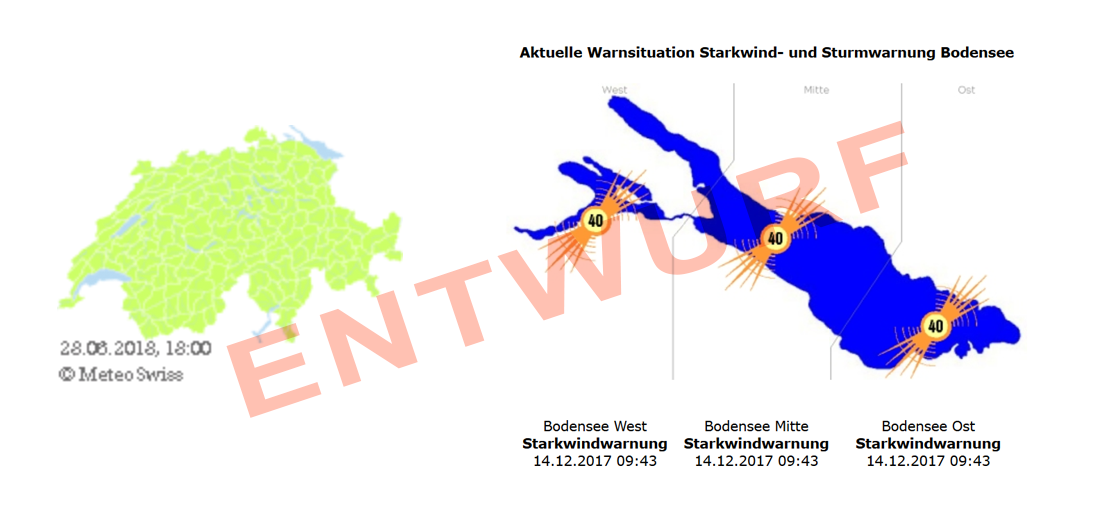
\includegraphics[width=1\linewidth]{img/sturm}
	\caption{Sturmwarnung vom Kanton Thurgau}
	\label{img:sturm}
\end{figure}

Wie schon erklärt ist das Problem hierbei der HTTP Standard, viele der Webbrowser stellen die Unterstützung dieses Standards langsam aber sicher ein und werden dann nur noch HTTPS unterstützen\cite{Mozilla:DeprecatingNon-SecureHTTP}. Deswegen ist die Sturmwarnung nur über einen Link aufrufbar. 